\documentclass[acmtog]{acmart}
\usepackage{subfigure}
\usepackage{listings}
\usepackage{bm}
\usepackage{amsmath}

\newcommand{\code}[1]{\texttt{\color{magenta}{#1}}}
\graphicspath{{img/}}

\definecolor{blve}{rgb}{0.3372549 , 0.61176471, 0.83921569}
\definecolor{gr33n}{rgb}{0.29019608, 0.7372549, 0.64705882}
\makeatletter
\lst@InstallKeywords k{class}{classstyle}\slshape{classstyle}{}ld
\makeatother
\lstset{language=C++,
	basicstyle=\ttfamily,
	keywordstyle=\radiance{blve}\ttfamily,
	stringstyle=\radiance{red}\ttfamily,
	commentstyle=\radiance{magenta}\ttfamily,
	morecomment=[l][\radiance{magenta}]{\#},
	classstyle = \bfseries\radiance{gr33n},
	tabsize=2
}
\lstset{basicstyle=\ttfamily}

% Title portion
\title{Final Project: {Ray Tracing Trimmed NURBS}}

\author{Name:\quad Zeen Chi, Wenchao Li  \\ student number:\ 2020533089, 2020533159
\\email:\quad \{chize, liwch1\}@shanghaitech.edu.cn}

% Document starts
\begin{document}
\maketitle

\vspace*{2 ex}

\section{Introduction}
\hspace*{8pt}
Computer Aided Design (CAD) modeling tools are widely used for the industrial design of models for prototyping and production. The standard surface representation within these systems are trimmed non-uniform rational B-Spline (NURBS) surfaces. Trimmed NURBS surfaces are capable of compactly describing almost any shape and additionally provide local and intuitive control. These patches are commonly visualized by rendering a triangle- based approximation (tessellation) on graphic processing units (GPU), since there is no specialized NURBS rendering hardware readily available. The process of generating a high-quality tessellation is time-consuming, especially for trimmed surfaces requiring fine sampling of the trim boundaries. Therefore, it is complicated to render a NURBS surface with both efficiency and accuracy.

In this final project, we implement a ray tracing system that can render an arbitrary NURBS surface without tessellation. The outline of our approach can be briefly described by Figure 1. We create a set of boxes that bound the underlying surface over a given parametric range. The ray is tested for intersection with these boxes, and for a particular box that is hit, a parametric value within the box is used to initiate root finding. The key issues are determining which boxes to use, how to efficiently manage computing intersections with them, how to do the root finding, and how to efficiently evaluate the geometry for a given parametric value.
We use refinement to generate the bounding volume hierarchy, which results in a shallower tree depth than other subdivision-based methods. We also use an efficient refinement-based point evaluation method to speed root-finding. These choices turn out to be both reasonable to implement and efficient.

In Section 2 we present the bulk of our method, in particular how to create a hierarchy of bounding boxes and how to perform root finding within a single box to compute an intersection with an untrimmed NURBS surface. In Section 3 we describe how to extend the method to trimmed NURBS surfaces, although in practice we have not implemented the last part yet. In Section 4 we will show the results of our implementation. Finally, in Section 5 we will briefly talk about our workload distribution.

As for the result, we render different NURBS surface models with different complexity. We found a duck model that consists of three NURBS patches and rendered it to justify the correctness and efficiency of the untrimmed NURBS rendering scheme. We also found some complex trimmed NURBS models, e.g. Eiffel Tower and a very intricate ring, to show the correctness of the trimmed NURBS surface rendering scheme.

\textbf{Note: the formulae derivation described in this report are not derived by us. We list them only to clarify the correctness of the corresponding formulae. However, every part of the algorithms described below is fully implemented by ourselves.}

\begin{figure}[t]
    \centering
    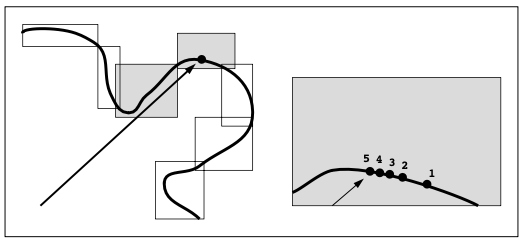
\includegraphics[width=0.4\textwidth]{overview.png}
    \caption{The basic method we use to find the intersection of a ray and a parametric object shown in a 2D example. Left: The ray is tested against a series of axis-aligned bounding boxes. Right: For each box hit an initial guess is generated in the parametric interval the box bounds. Root finding is then iteratively applied until a convergence or a divergence criterion is met.}
\end{figure}

\section{Untrimmed NURBS Surfaces Rendering}
\subsection{Basic Formulations}
\hspace*{8pt}
A NURBS surface can be formulated by
\[
    \mathbf{S}^w(u,v)=\sum_{i=0}^{M-1}\sum_{j=0}^{N-1}\mathbf{P}^w_{i,j}B_{j,k_u}(u)B_{i,k_v}(v)
\]
where the superscript $w$ denotes that our formulation produces a point in rational four space, which must be normalized by the homogeneous coordinate prior to display. The $\{\mathbf{P}_{i,j}^w\}_{i=0,j=0}^{M-1,N-1}$ are the control points $(w_{i,j}x_{i,j},w_{i,j}y_{i,j},w_{i,j}z_{i,j},w_{i,j})$ of the $M\times N$ mesh, having basis functions $B_{j,k_u}$ and $B_{i,k_v}$ of orders $k_u$ and $k_v$ respectively defined over knot vectors
\[
    \begin{split}
        \tau_u=\{u_j\}_{j=0}^{N-1+k_u}\\
        \tau_v=\{v_j\}_{j=0}^{M-1+k_v}
    \end{split}    
\]
and the basis functions are formulated by
\[
    \begin{split}
        B_{j,k_u}(u)&=\begin{cases}
            1&\text{if }k_u=1\text{ and }u\in[u_j,u_{j+1})\\
            0&\text{if }k_u=1\text{ and }u\notin[u_j,u_{j+1})\\
            \frac{u-u_j}{u_{j+k_u-1}-u_j}B_{j,k_u-1}(u)+\\
            \frac{u_{j+k_u}-u}{u_{j+k_u}-u_{j+1}}B_{j+1,k_u-1}(u)&\text{otherwise}
        \end{cases}\\
        B_{i,k_v}(v)&=\begin{cases}
            1&\text{if }k_v=1\text{ and }v\in[v_j,v_{j+1})\\
            0&\text{if }k_v=1\text{ and }v\notin[v_j,v_{j+1})\\
            \frac{v-v_i}{v_{i+k_v-1}-v_i}B_{i,k_v-1}(v)+\\
            \frac{v_{i+k_v}-v}{v_{i+k_v}-v_{i+1}}B_{i+1,k_v-1}(u)&\text{otherwise}
        \end{cases}
    \end{split}
\]
For a ray tracer, a ray is defined by:
\[
    \mathbf{r}(t)=\mathbf{o}+\hat{\mathbf{d}}\times t
\]
but we need to rewrite it as the intersection of two orthogonal planes $\{\mathbf{p}\ |\ \mathbf{P}_1\cdot(\mathbf{p},1)=0\}$ and $\{\mathbf{p}\ |\ \mathbf{P}_2\cdot(\mathbf{p},1)=0\}$, where $\mathbf{P}_1=(\mathbf{N}_1,d_1)$ and $\mathbf{P}_2=(\mathbf{N}_2,d_2)$, and $d_1$ and $d_2$ are the distances from the plane to the world origin, respectively. The normal to the plane is defined as
\[
    \mathbf{N}_1=\begin{cases}
        (\hat{\mathbf{d}}_y,-\hat{\mathbf{d}}_x,0)&\text{if }|\hat{\mathbf{d}}_x|>|\hat{\mathbf{d}}_y|\text{ and }|\hat{\mathbf{d}}_x|>|\hat{\mathbf{d}}_z|\\
        (0,\hat{\mathbf{d}}_z,-\hat{\mathbf{d}}_y)&\text{otherwise}
    \end{cases}
\]
and $\mathbf{N}_2$ is simply
\[
    \mathbf{N}_2=\mathbf{N}_1\times\hat{\mathbf{d}}
\]
and $d_1$ and $d_2$ can be calculated by
\[
    \begin{split}
        d_1&=-\mathbf{N}_1\cdot\mathbf{o}\\
        d_2&=-\mathbf{N}_2\cdot\mathbf{o}
    \end{split}
\]
The representation of the ray as two orthogonal planes is shown in Figure 2.
\begin{figure}[htbp]
    \centering
    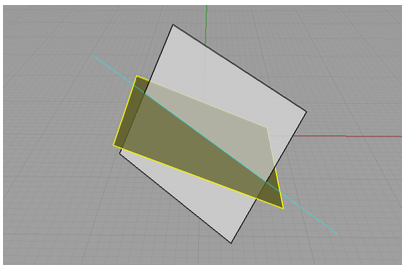
\includegraphics[width=0.4\textwidth]{ray.png}
    \caption{The plane-intersection representation of a ray}
\end{figure}
\subsection{Root Finder}
\hspace*{8pt}
Given a ray as the intersection of planes $\mathbf{P}_1=(\mathbf{N}_1,d_1)$ and $\mathbf{P}_2=(\mathbf{N}_2,d_2)$, we need to find the root $(u_*,v_*)$ of
\[
    \mathbf{F}(u,v)=\begin{pmatrix}
        \mathbf{N}_1\cdot\mathbf{S}(u,v)+d_1\\
        \mathbf{N}_2\cdot\mathbf{S}(u,v)+d_2
    \end{pmatrix}
\]

We take Newton's method as the root finder for some reasons. First, it converges quadratically if the initial guess is close, which we ensure by constructing a bounding volume hierarchy. Furthermore, the surface derivatives exist and are calculated at cost comparable to that of surface evaluation. This means that there is likely little computational advantage to utilizing approximate derivative methods such as Broyden.

For each iteration of Newton's method, the update rule is
\[
    \begin{pmatrix}
        u_{n+1}\\
        v_{n+1}
    \end{pmatrix}
    =
    \begin{pmatrix}
        u_{n}\\
        v_{n}
    \end{pmatrix}
    -\mathbf{J}^{-1}(u_n,v_n)\cdot\mathbf{F}(u_n,v_n)
\]
where $\mathbf{J}$ is the Jacobian matrix of $\mathbf{F}$, which is
\[
    \mathbf{J}=\begin{pmatrix}
        \mathbf{N}_1\cdot\mathbf{S}_{\mathbf{u}}(u,v)&\mathbf{N}_1\cdot\mathbf{S}_{\mathbf{v}}(u,v)\\
        \mathbf{N}_2\cdot\mathbf{S}_{\mathbf{u}}(u,v)&\mathbf{N}_2\cdot\mathbf{S}_{\mathbf{v}}(u,v)
    \end{pmatrix}
\]

There are four terminating criteria. For the success criterion, which is, if we are closer to the root than a threshold $\epsilon$, i.e.,
\[
    \lVert\mathbf{F}(u_n,v_n)\rVert<\epsilon
\]
then we report a hit. Otherwise, we should report a miss. We do not allow the new $(u_*,v_*)$ estimate to take us further from the root than the previous one:
\[
    \lVert\mathbf{F}(u_{n+1},v_{n+1})\rVert>\lVert\mathbf{F}(u_n,v_n)\rVert
\]

We also do not allow the iteration to take us outside the parametric domain of the surface:
\[
    u\notin[u_{k_u-1},u_N),v\notin[v_{k_v-1},v_M)
\]

And we limit the number of iterations to $N_{\text{max}}=MAXITER$, which is set as 7 by practice.

A final check is made to assure that the Jacobian matrix $\mathbf{J}$ is not singular. While this would seem to be a rare occurrence in theory, we have encountered this problem in practice. In the situation where $\mathbf{J}(u_k,v_k)$ is singular, either the surface is not regular $(\mathbf{S}_{\mathbf{u}} \times \mathbf{S}_{\mathbf{v}} = 0)$ or the ray is parallel to a silhouette ray at the point $\mathbf{S}(u_k , v_k)$. In either situation, to determine singularity, we test
\[|\mathrm{det}(\mathbf{J})|<\epsilon\]

If the Jacobian matrix is singular, we perform a jittered perturbation of the parametric evaluation point, i.e.,
\[
    \begin{pmatrix}
        u_{n+1}\\
        v_{n+1}
    \end{pmatrix}
    =
    \begin{pmatrix}
        u_{n}\\
        v_{n}
    \end{pmatrix}
    +0.1\times
    \begin{pmatrix}
        \mathrm{rand}(0,1)\times(u_0-u_k)\\
        \mathrm{rand}(0,1)\times(v_0-v_k)
    \end{pmatrix}
\]
to initiate the next iteration, where $(u_0,v_0)$ is the initial guess of the root.

\subsection{NURBS Surface Subdivision}
\hspace*{8pt}
For Newton to converge both swiftly and reliably, the initial guess must be suitably close to the actual root. We employ a flattening procedure, i.e., refining/subdividing the control mesh so that each span meets some flatness criteria — both to ensure that the initial guess is a good one, and for the purpose of generating a bounding volume hierarchy for ray culling.

We utilize the curvature-based refinement of the knot vectors, which will be described below.

Suppose we have a B-spline curve $c(t)$. An oracle for determining the extent to which the span $[t_i , t_{i+1})$ should be refined is given by the product of its maximum curvature and its length over that span. Long curve segments should be divided in order to ensure that the initial guess for the numerical solver is reasonably close to the actual root. High curvature regions should be split to avoid multiple roots. As we are utilizing maximum curvature as a measure of flatness, our heuristic will be overly conservative for curves other than circles. The heuristic value for the number of knots to add to the current span is given by
\[
    n_1=C_1 * \max _{\left[t_i, t_{i+1}\right)}\{\operatorname{curvature}(\mathbf{c}(t))\} * \operatorname{arclen}(\mathbf{c}(t))_{\left[t_i, t_{i+1}\right)} \text {. }
\]

We also choose to bound the deviation of the curve from its linear approximation. This notion will imbue our heuristic with scale dependence. Thus, for example, large circles will be broken into more pieces than small circles. Erring again on the conservative side, suppose our curve span is a circle with radius r, which we are approximating with linear segments. A measure of the accuracy of the approximation can be phrased in terms of a chord height h which gives the maximum deviation of the facets from the circle. Observing Figure 3, it can be seen that
\[
    \begin{aligned}
        h & =r-d \\
        & =r-r \cos \frac{\theta}{2} \\
        & \approx r\left(1-\left(1-\frac{\theta^2}{8}\right)\right) \\
        & =\frac{r \theta^2}{8} .
    \end{aligned}
\]
The number of segments n2 required to produce a curve within this tolerance is computed by $2\pi/\theta$. Thus, we have
\[
    \begin{aligned}
        n_2 &=\frac{2 \pi}{\sqrt{\frac{8 h}{r}}} \\
        & =\frac{2 \pi \sqrt{r}}{\sqrt{8 h}} \\
        & \approx C_2 * \sqrt{\mathrm{arclen}(\mathbf{c}(t))_{[t_i, t_{i+1})}}
    \end{aligned}
\]
\begin{figure}
    \centering
    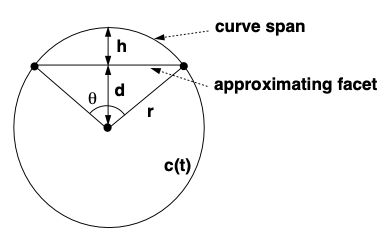
\includegraphics[width=0.4\textwidth]{heu.png}
    \caption{Illustration of the chord height tolerance heuristic.}
\end{figure}

Combining the preceding oracles for curve behavior, our heuristic for the number of knots n to add to an interval will be $n_1*n_2$:
\[
    n=C * \max _{\left[t_i, t_{i+1}\right)}\{\operatorname{curvature}(\mathbf{c}(t))\} * \operatorname{arclen}(\mathbf{c}(t))_{\left[t_i, t_{i+1}\right)}^{3 / 2}
\]
where we set $C=35$ in practice.

After a set of intricate approximations, the formula above can be rewritten as
\[
    \begin{aligned}
        n & =C * \frac{\max _{\left[t_i, t_{i+1}\right)}\left\{\left|\mathbf{c}^{\prime \prime}(t)\right|\right\} *\left[\operatorname{avg}_{\left[t_i, t_{i+1}\right)}\left\{\left|\mathbf{c}^{\prime}(t)\right|\right\} *\left(t_{i+1}-t_i\right)\right]^{3 / 2}}{\operatorname{avg}_{\left[t_i, t_{i+1}\right)}\left\{\left|\mathbf{c}^{\prime}(t)\right|\right\}^2} \\
        & =C * \frac{\max_{\left[t_i, t_{i+1}\right)}\left\{\left|\mathbf{c}^{\prime \prime}(t)\right|\right\} *\left(t_{i+1}-t_i\right)^{3 / 2}}{\operatorname{avg}_{\left[t_i, t_{i+1}\right)}\left\{\left|\mathbf{c}^{\prime}(t)\right|\right\}^{1 / 2}} \\
        & =C * \frac{\max _{i-k+3 \leq j \leq i}\left\{\left|\mathbf{A}_{\mathbf{j}}\right|\right\}\left(t_{i+1}-t_i\right)^{3 / 2}}{\left(\frac{1}{k-1} \sum_{j=i-k+2}^i\left|\mathbf{V}_{\mathbf{j}}\right|\right)^{1 / 2}} .
        \end{aligned}
\]
where $\mathbf{V}_{\mathbf{j}}=(k-1) \frac{\left(\mathbf{P}_{\mathbf{j}}-\mathbf{P}_{\mathbf{j}-\mathbf{1}}\right)}{t_{j+k-1}-t_j}$ and $\mathbf{A}_{\mathbf{j}}=(k-2) \frac{\left(\mathbf{V}_{\mathbf{j}}-\mathbf{V}_{\mathbf{j}-1}\right)}{t_{j+k-2}-t_j}$.

For each row of the mesh, we apply the above heuristic to calculate how many knots need to be added to each $u$ knot interval, the final number being the maximum across all rows. This process is repeated for each column in order to refine the $v$ knot vector. The inserted knots are spaced uniformly within the existing knot intervals.

As a final step in the flattening routine, we "close" all of the knot intervals in the refined knot vectors $\mathbf{t}_{\mathbf{u}}$ and $\mathbf{t}_{\mathbf{v}}$. By this, we mean that we give multiplicity $k_u-1$ to each internal knot of $\mathbf{t}_{\mathbf{u}}$ and multiplicity $k_u$ to each end knot. Similarly, we give multiplicities of $k_v-1$ and kv to the internal and external knots, respectively, of $\mathbf{t}_{\mathbf{v}}$. The result is a Bezier surface patch corresponding to each non-empty interval $[u_i,u_{i+1})\times[v_j,v_{j+1})$ of $\mathbf{t}_{\mathbf{u}}\times\mathbf{t}_{\mathbf{v}}$,which we can bound using the convex hull of the corresponding refined surface mesh points.

\subsection{Bounding Volume Hierarchy (BVH)}
\hspace*{8pt}
We build a bounding volume hierarchy using the points of the refined control mesh we found in the previous section. The root and internal nodes of the tree will contain simple primitives which bound portions of the underlying surface. The leaves of the tree are special objects, which we call interval objects, are used to provide an initial guess (in our case, the midpoint of the bracketing parametric interval) to the Newton iteration. We will now examine the specifics in more detail.

The convex hull property of B-spline surfaces guarantees that the surface is contained in the convex hull of its control mesh. As a result, any convex objects which bound the mesh will bound the underlying surface. We can actually make a stronger claim. Since we closed the knot intervals in the last section [made the multiplicity of the internal knots $k-1$], each non-empty interval $[u_i,u_{i+1})\times[v_j,v_{j+1})$ corresponds to a surface patch which is completely contained in the convex hull of its corresponding mesh points. Thus, if we produce an axis-aligned bounding box (AABB) for each of these intervals, we will have completely enclosed the surface. This is the basic idea behind the bounding volume hierarchy we use in our implementation.

\subsection{KD-Tree}
\hspace*{8pt}
In spite of BVH, we also built a kd-tree as the acceleration structure. The kd-tree is a binary tree, where each node is a hyperplane that splits the space into two subspaces. The kd-tree is constructed by recursively partitioning the space into two subspaces. The splitting hyperplane is chosen following the Surface-Area Heuristics (SAH) function. The kd-tree is used to accelerate the intersection test between the ray and the AABBs. The leaf nodes of kd-tree contains multiple AABBs, which is already elaborated in the above subsection. The intersection test is performed by traversing the kd-tree. At each node, the ray is tested against the splitting hyperplane. If the ray intersects the splitting hyperplane, the ray is tested against the two subspaces recursively. Once the traversal comes to the leaf node, we perform intersection test with the ray and the corresponding AABBs, then return the closest intersection point.

In section 3, we will compare the speed and accuracy of BVH and KD-Tree, to find out which acceleration structure is better for the NURBS surface intersection situation.

\subsection{Refined Control Points Evaluation}
\hspace*{8pt}
We need to elaborate how to generate the refined control points $\mathbf{D}_i^{\omega}$. We again formulate our solution in the context of curves, and then generalize the result to surfaces.

Earlier we proposed to evaluate the curve $\mathbf{c}$ at $t_*$ by stacking $k-1 \ t_*$-valued knots in its knot vector $\tau$ to generate the refined knot vector $\mathbf{t}$. The B-Spline basis transformation defined by this refinement yields a matrix $\mathbf{A}$ which can be used to calculate the refined control polygon $\mathbf{D}^\omega$ from the original polygon $\mathbf{P}^{\mathbf{w}}$ :
$$
\mathbf{D}^\omega=\mathbf{A} \mathbf{P}^{\mathbf{w}}.
$$
We are not interested in calculating the full alpha matrix $\mathbf{A}$, but merely rows $\mu-k+2$ and $\mu-k+1$, as these are used to generate the points $\mathbf{D}_{\mu-\mathbf{k}+\mathbf{2}}^\omega$ and $\mathbf{D}_{\mu-\mathbf{k + 1}}^\omega$ which are required for point and derivative evaluation.
Suppose $t_* \in\left[\tau_{\mu^{\prime}}, \tau_{\mu^{\prime}+1}\right)$. We can generate the refinement for row $\mu+k-1$ using a triangular scheme
$$
\begin{array}{rcc} 
& & \alpha_{\mu^{\prime}, 0}^{\prime} \\
& \alpha_{\mu^{\prime}-1,1}^{\prime} & \alpha_{\mu^{\prime}, 1}^{\prime} \\
& \vdots & \vdots \\
\alpha_{\mu^{\prime}-\nu, \nu}^{\prime} & \cdots & \alpha_{\mu^{\prime}, \nu}^{\prime}
\end{array}
$$
where $\nu$ is the number of knots we are inserting and
$$
\begin{aligned}
\alpha_{j, 1}^{\prime} & =\delta_{j, \mu^{\prime}} \\
\alpha_{j, p+1}^{\prime} & =\gamma_{j, p} \alpha_{j, p}^{\prime}+\left(1-\gamma_{j+1, p}\right) \alpha_{j+1, p}^{\prime} \\
\gamma_{j, p} & = \begin{cases}\left(t_*-\tau_{\mu^{\prime}-p+j-(k-1-\nu)}\right) / d, & \text { if } d=\tau_{\mu^{\prime}+1+j}-\\&\tau_{\mu^{\prime}-p+j-(k-1-\nu)}>0 \\
\text { arbitrary } & \text { otherwise. }\end{cases}
\end{aligned}
$$
$\mathbf{A}_{\mu-k+1, j}=\alpha_{j, \nu}^{\prime}$ for $j=\mu^{\prime}-\nu, \cdots, \mu^{\prime}$ and $\mathbf{A}_{i, j}=0$ otherwise. If $n$ knots exist in the original knot vector $\tau$ with value $t_*$, then $\nu=\max \{k-1-n, 1\}$ - that is to say, we always insert at least 1 knot. The quantity $\nu$ is used in the triangular scheme above to allow one to skip those basis functions which are trivially 0 or 1 due to repeated knots. As a result of this triangular scheme, we generate basis functions in place and avoid redundant computation of $\alpha^{\prime}$ values for subsequent levels.

In the refinement scheme we propose, the point on the curve $\mathbf{D}_{\mu-\mathbf{k}+\mathbf{1}}^\omega$ will be a convex blend of the points $\mathbf{D}_{\mu-\mathbf{k}}^\omega$ and $\mathbf{D}_{\mu-\mathbf{k}+\mathbf{2}}^\omega$. The blend factor will be $\gamma_{\mu^{\prime}, 0}$. The factor $\gamma_{\mu^{\prime}, 0}$ is introduced at the first level of the recurrence. The leaf terms can be written as
$$
\alpha_{j, \nu}^{\prime}=\left(1-\gamma_{\mu^{\prime}, 0}\right) l_{j, \nu}+\gamma_{\mu^{\prime}, 0} r_{j, \nu}
$$
with $j=\mu^{\prime}-\nu, \cdots, \mu^{\prime} .\left\{l_{j, \nu}\right\}$ and $\left\{r_{j, \nu}\right\}$ are those terms dependent on $\alpha_{\mu-1,1}^{\prime}$ and $\alpha_{\mu, 1}^{\prime}$ respectively. They are the elements of the alpha matrix rows $\mu-k$ and $\mu-k+2$ with $\mathbf{A}_{\mu-k, j}=l_{j, \nu}$ and $\mathbf{A}_{\mu-k+2, j}=r_{j, \nu}$ for $j=\mu^{\prime}-\nu, \cdots, \mu^{\prime}$. We can generate the $\left\{l_{j, \nu}\right\}$ by setting $\alpha_{\mu^{\prime}-1,1}^{\prime}=1$ and $\alpha_{\mu^{\prime}, 1}^{\prime}=0$ and likewise, generate $\left\{r_{j, \nu}\right\}$ by setting $\alpha_{\mu^{\prime}-1,1}^{\prime}=0$ and $\alpha_{\mu^{\prime}, 1}^{\prime}=1$. Thus, $\mathbf{A}_{\mu-k, j}$ and $\mathbf{A}_{\mu-k+2, j}$ can be generated in the course of generating $\mathbf{A}_{\mu-k+1, j}$ at little additional expense.

The procedure above generalizes easily to surfaces, allowing us to generate the desired rows of the refinement matrices $\mathbf{A}_{\mathbf{u}}$ and $\mathbf{A}_{\mathbf{v}}$. The refined mesh $\mathbf{D}^\omega$ is derived from the existing mesh $\mathbf{P}^{\mathbf{w}}$ by:
$$
\mathbf{D}^\omega=\mathbf{A}_{\mathbf{u}} \mathbf{P}^{\mathbf{w}} \mathbf{A}_{\mathbf{v}}^{\mathbf{T}}
$$
To produce the desired points we only need to evaluate
$$
\begin{aligned}
& \left(\begin{array}{ll}
\mathbf{D}_{\mu_{\mathbf{u}}-\mathbf{k}_{\mathbf{u}}+\mathbf{1}, \mu_{\mathbf{v}}-\mathbf{k}_{\mathbf{v}}+\mathbf{1}}^\omega & \mathbf{D}_{\mu_{\mathbf{u}}-\mathbf{k}_{\mathbf{u}}+\mathbf{1}, \mu_{\mathbf{v}}-\mathbf{k}_{\mathbf{v}}+\mathbf{2}}^\omega \\
\mathbf{D}_{\mu_{\mathbf{u}}-\mathbf{k}_{\mathbf{u}}+\mathbf{2}, \mu_{\mathbf{v}}-\mathbf{k}_{\mathbf{v}}+\mathbf{1}}^\omega & \mathbf{D}_{\mu_{\mathbf{u}}-\mathbf{k}_{\mathbf{u}}+\mathbf{2}, \mu_{\mathbf{v}}-\mathbf{k}_{\mathbf{v}}+\mathbf{2}}^\omega
\end{array}\right)= \\
& \left(\begin{array}{l}
\left(\mathbf{A}_{\mathbf{u}}\right)_{\mu_u+k_u+1,\left[\mu_u^{\prime}-\nu_u \ldots \mu_u^{\prime}\right]} \\
\left(\mathbf{A}_{\mathbf{u}}\right)_{\mu_u+k_u+2,\left[\mu_u^{\prime}-\nu_u \ldots \mu_u^{\prime}\right]}
\end{array}\right) \mathbf{P}_{\left[\mu_{\mathbf{u}}^{\prime}-\nu_{\mathbf{u}} \ldots \mu_{\mathbf{u}}^{\prime}\right]\left[\mu_{\mathbf{v}}^{\prime}-\nu_{\mathbf{v}} \ldots \mu_{\mathbf{v}}^{\prime}\right]}^{\mathbf{w}}\\
&\left(\begin{array}{c}
\left(\mathbf{A}_{\mathbf{v}}\right)_{\mu_v+k_v+1,\left[\mu_v^{\prime}-\nu_v \ldots \mu_v^{\prime}\right]} \\
\left(\mathbf{A}_{\mathbf{v}}\right)_{\mu_v+k_v+2,\left[\mu_v^{\prime}-\nu_v \ldots \mu_v^{\prime}\right]}
\end{array}\right)^T
\end{aligned}
$$
After that, the entrices of matrix
\[
\begin{aligned}
    \left(\begin{array}{ll}
        \mathbf{D}_{\mu_{\mathbf{u}}-\mathbf{k}_{\mathbf{u}}+\mathbf{1}, \mu_{\mathbf{v}}-\mathbf{k}_{\mathbf{v}}+\mathbf{1}}^\omega & \mathbf{D}_{\mu_{\mathbf{u}}-\mathbf{k}_{\mathbf{u}}+\mathbf{1}, \mu_{\mathbf{v}}-\mathbf{k}_{\mathbf{v}}+\mathbf{2}}^\omega \\
        \mathbf{D}_{\mu_{\mathbf{u}}-\mathbf{k}_{\mathbf{u}}+\mathbf{2}, \mu_{\mathbf{v}}-\mathbf{k}_{\mathbf{v}}+\mathbf{1}}^\omega & \mathbf{D}_{\mu_{\mathbf{u}}-\mathbf{k}_{\mathbf{u}}+\mathbf{2}, \mu_{\mathbf{v}}-\mathbf{k}_{\mathbf{v}}+\mathbf{2}}^\omega
    \end{array}\right)
\end{aligned}
\]
will be utilized by the NURBS surface derivatives and normal vectors evaluation described in the next section.

\subsection{Derivatives and Normal Evaluation}
\hspace*{8pt}
The Newton iteration requires us to perform surface and derivative evaluation at a point $(u, v)$ on the surface. In this section we examine how this can be accomplished efficiently. We begin by examining the problem in the context of B-spline curves. We then generalize the result to surfaces.

We evaluate a curve $\mathbf{c}(t)$ by using refinement to stack $k-1$ knots (where $k$ is the order of the curve) at the desired parameter value $t_*$. The refined curve is defined over a new knot vector $\mathbf{t}$ with basis functions $N_{i, k}(t)$ and new control points $\omega_i \mathbf{D}_i$. Recall the recurrence for the B-Spline basis functions:
$$
N_{i, k}(t)=\left\{\begin{array}{cl}
1 & \text { if } k=1 \text { and } t \in\left[t_i, t_{i+1}\right) \\
0 & \text { if } k=1 \text { and } t \notin\left[t_i, t_{i+1}\right) \\
\frac{t-t_i}{t_{i+k-1}-t_i} N_{i, k-1}(t)+\\
\frac{t_{i+k}-t}{t_{i+k}-t_{i+1}} N_{i+1, k-1}(t) & \text { otherwise. }
\end{array}\right.
$$
Let $t_* \in\left[t_\mu, t_{\mu+1}\right)$. As a result of refinement, $t_*=t_\mu=\ldots=t_{\mu-k+2}$. According to the definition of the basis functions, $N_{\mu, 1}\left(t_*\right)=1$. There are only two potentially non-zero basis functions of order $k=2$, namely those dependent on $N_{\mu, 1}: N_{\mu, 2}$ and $N_{\mu-1,2}$. From the recurrence,
$$
\begin{aligned}
N_{\mu, 2}\left(t_*\right) & =\frac{t_*-t_\mu}{t_{\mu+k-1}-t_\mu} N_{\mu, 1}\left(t_*\right)+\frac{t_{i+k}-t_*}{t_{\mu+k}-t_{\mu+1}} N_{\mu+1,1}\left(t_*\right) \\
& =0 * 1+\frac{t_{i+k}-t_*}{t_{\mu+k}-t_{\mu+1}} * 0 \\
& =0
\end{aligned}
$$
and,
$$
\begin{aligned}
N_{\mu-1,2}\left(t_*\right) & =\frac{t_*-t_{\mu-1}}{t_{\mu+k-2}-t_{\mu-1}} N_{\mu-1,1}\left(t_*\right)+\frac{t_{\mu+k-1}-t_*}{t_{\mu+k-1}-t_\mu} N_{\mu, 1}\left(t_*\right) \\
& =0 * 0+1 * 1 \\
& =1 .
\end{aligned}
$$

Likewise, the only non-zero order $k=3$ terms will be those dependent on $N_{\mu-1,2}: N_{\mu-1,3}$ and $N_{\mu-2,3}$.
$$
\begin{aligned}
N_{\mu-1,3}\left(t_*\right) & =\frac{t_*-t_{\mu-1}}{(\cdots)} * 1+(\cdots) * 0 \\
& =0 \\
N_{\mu-2,3}\left(t_*\right) & =(\cdots) * 0+\frac{t_{\mu-2+k}-t_*}{t_{\mu-2+k}-t_{\mu-1}} * 1 \\
& =1
\end{aligned}
$$

The pattern that emerges is that $N_{\mu-k+1, k}\left(t_*\right)=1$. A straightforward consequence of this result is
$$
\mathbf{c}\left(t_*\right)=\frac{\sum_i N_{i, k}\left(t_*\right) \omega_i \mathbf{D}_{\mathbf{i}}}{\sum_i N_{i, k}\left(t_*\right) \omega_i}=\frac{\omega_{\mu-k+1} \mathbf{D}_{\mu-\mathbf{k}+\mathbf{1}}}{\omega_{\mu-k+1}}=\mathbf{D}_{\mu-\mathbf{k}+\mathbf{1}} .
$$

The point with index $\mu-k+1$ in the refined control polygon yields the point on the curve.
A further analysis can be used to yield the derivative. Given a rational curve
$$
\mathbf{c}(t)=\frac{\sum_i N_{i, k}(t) \omega_i \mathbf{D}_{\mathbf{i}}}{\sum_i N_{i, k}(t) \omega_i}=\frac{\sum_i N_{i, k}(t) \mathbf{D}_{\mathbf{i}}^\omega}{\sum_i N_{i, k}(t) \omega_i}=\frac{\mathbf{D}(t)}{\omega(t)},
$$
where $\mathbf{D}_{\mathbf{i}}^\omega=\omega_i \mathbf{D}_{\mathbf{i}}$, the derivative is given by the quotient rule
$$
\mathbf{c}^{\prime}(t)=\frac{\omega(t)\left(\mathbf{D}^\omega\right)^{\prime}(t)-\mathbf{D}^\omega(t) \omega^{\prime}(t)}{\omega(t)^2}
$$

By the preceding analysis $\mathbf{D}^\omega\left(t_*\right)=\mathbf{D}_{\mu-\mathbf{k}+\mathbf{1}}^\omega$. Likewise, $\omega\left(t_*\right)=\omega_{\mu-k+1}$. The derivative of the B-Spline basis function is given by
$$
N_{i, k}^{\prime}(t)=(k-1)\left[\frac{N_{i, k-1}(t)}{t_{i+k-1}-t_i}-\frac{N_{i+1, k-1}(t)}{t_{i+k}-t_{i+1}}\right] .
$$

Evaluating the derivative at $t_*$, we have
$$
\begin{aligned}
\left(\mathbf{D}^\omega\right)^{\prime}\left(t_*\right) & =\sum_i N_{i, k}^{\prime}\left(t_*\right) \mathbf{D}_i^\omega \\
& =(k-1) \sum_i \mathbf{D}_i^\omega\left(\frac{N_{i, k-1}\left(t_*\right)}{t_{i+k-1}-t_i}-\frac{N_{i+1, k-1}\left(t_*\right)}{t_{i+k}-t_{i+1}}\right) \\
& =(k-1)\left[\sum_i \mathbf{D}_i^\omega \frac{N_{i, k-1}\left(t_*\right)}{t_{i+k-1}-t_i}-\sum_i \mathbf{D}_i^\omega \frac{N_{i+1, k-1}\left(t_*\right)}{t_{i+k}-t_{i+1}}\right] .
\end{aligned}
$$

We know the only non-zero basis function of order $k-1$ is

$N_{\mu-k+2, k-1}\left(t_*\right)=1$. Therefore,
$$
\left(\mathbf{D}^\omega\right)^{\prime}\left(t_*\right)=(k-1)\left[\frac{\mathbf{D}_{\mu-\mathbf{k}+\mathbf{2}}^\omega}{t_{\mu+1}-t_{\mu-k+2}}-\frac{\mathbf{D}_{\mu-\mathbf{k}+\mathbf{1}}^\omega}{t_{\mu+1}-t_{\mu-k+2}}\right]
$$
Analogously,
$$
\omega^{\prime}\left(t_*\right)=(k-1)\left[\frac{\omega_{\mu-k+2}}{t_{\mu+1}-t_{\mu-k+2}}-\frac{\omega_{\mu-k+1}}{t_{\mu+1}-t_{\mu-k+2}}\right]
$$
Plugging in for $\mathbf{c}^{\prime}(t)$
$$
\begin{aligned}
\mathbf{c}^{\prime}\left(t_*\right) & =(k-1)\left[\frac{\frac{\mathbf{D}_{\mu-\mathbf{k}+2}^\omega-\mathbf{D}_{\mu-\mathbf{k}+\mathbf{1}}^\omega}{t_{\mu+1}-t_{\mu-k+2}} \omega_{\mu-k+1}-\mathbf{D}_{\mu-\mathbf{k}+\mathbf{1}}^\omega \frac{\omega_{\mu-k+2}-\omega_{\mu-k+1}}{t_{\mu+1}-t_{\mu-k+2}}}{\omega_{\mu-k+1}^2}\right] \\
& =\frac{k-1}{\left(t_{\mu+1}-t_{\mu-k+2}\right) \omega_{\mu-k+1}}\left[\mathbf{D}_{\mu-\mathbf{k + 2}}^\omega-\mathbf{D}_{\mu-\mathbf{k}+\mathbf{1}}^\omega \frac{\omega_{\mu-k+2}}{\omega_{\mu-k+1}}\right] \\
& =\frac{(k-1) \omega_{\mu-k+2}}{\left(t_{\mu+1}-t_*\right) \omega_{\mu-k+1}}\left[\mathbf{D}_{\mu-\mathbf{k}+\mathbf{2}}-\mathbf{D}_{\mu-\mathbf{k}+\mathbf{1}}\right] .
\end{aligned}
$$

The result for surface evaluation follows directly from the curve derivation, due to the independence of the parameters in the tensor product, so we shall simply state the results:
$$
\begin{aligned}
\mathbf{S}\left(u_*, v_*\right) & =\mathbf{D}_{\mu_{\mathbf{u}}-\mathbf{k}_{\mathbf{u}}+\mathbf{1}, \mu_{\mathbf{v}}-\mathbf{k}_{\mathbf{v}}+\mathbf{1}} \\
\mathbf{S}_{\mathbf{u}}\left(u_*, v_*\right) & =\frac{\left(k_u-1\right) \omega_{\mu_u-k_u+2, \mu_v-k_v+1}}{\left(u_{\mu_u+1}-u_*\right) \omega_{\mu_u-k_u+1, \mu_v-k_v+1}}\times \\
&\left[\mathbf{D}_{\mu_{\mathbf{u}}-\mathbf{k}_{\mathbf{u}}+\mathbf{2}, \mu_{\mathbf{v}}-\mathbf{k}_{\mathbf{v}}+\mathbf{1}}-\mathbf{D}_{\mu_{\mathbf{u}}-\mathbf{k}_{\mathbf{u}}+\mathbf{1}, \mu_{\mathbf{v}}-\mathbf{k}_{\mathbf{v}}+\mathbf{1}}\right] \\
\mathbf{S}_{\mathbf{v}}\left(u_*, v_*\right) & =\frac{\left(k_v-1\right) \omega_{\mu_u-k_u+1, \mu_v-k_v+2}}{\left(v_{\mu_v+1}-v_*\right) \omega_{\mu_u-k_u+1, \mu_v-k_v+1}}\times\\
&\left[\mathbf{D}_{\mu_{\mathbf{u}}-\mathbf{k}_{\mathbf{u}}+\mathbf{1}, \mu_{\mathbf{v}}-\mathbf{k}_{\mathbf{v}}+\mathbf{2}}-\mathbf{D}_{\mu_{\mathbf{u}}-\mathbf{k}_{\mathbf{u}}+\mathbf{1}, \mu_{\mathbf{v}}-\mathbf{k}_{\mathbf{v}}+\mathbf{1}}\right]
\end{aligned}
$$
The normal $\mathbf{n}(u, v)$ is given by the cross product of the first order partials:
$$
\mathbf{n}\left(u_*, v_*\right)=\mathbf{S}_{\mathbf{u}}\left(u_*, v_*\right) \times \mathbf{S}_{\mathbf{v}}\left(u_*, v_*\right)
$$
After getting the normal and derivatives, we can easily render the entire NURBS surface under a path tracer together with global illumination.

\textbf{Until now, we have fully elaborated all the algorithms needed. As long as combining all of them appropriately, we can successfully render the untrimmed NURBS surface using a ray tracer without tessellating the surface.}

\section{Trimmed NURBS surface rendering}
\hspace*{8pt}
Trimming curves are a common method for overcoming the topologically rectangular limitations of NURBS surfaces. They re- sult typically when designers wish to remove sections from models which are not aligned with the underlying parameterization. In this section, we will define what we mean by trimming curves.

A trimming curve is a closed, oriented curve which lies on a NURBS surface. For our purposes, the curve will consist of piecewise linear segments in parametric space $\left\{\mathbf{p}_{\mathbf{i}}=\left(u_i, v_i\right)\right\}$. In real-world model, a single looped trimming curve may consist of multiple curve segments, whose control points are end to end.

We calculate the orientation of the curve using the method of Rokne for computing the area of a polygon. Given parametric points $\left\{\mathbf{p}_{\mathbf{i}}=\left(u_i, v_i\right)\right\}, i=0 \ldots n$, the signed area can be computed by
$$
A=\frac{1}{2} \sum_{i=0}^n u_i v_{(i+1) \bmod n}-u_{(i+1) \bmod n} v_i .
$$
If $A$ is negative, the curve has a clockwise orientation. Otherwise, the orientation is counter-clockwise. The orientation of a trimming curve determines which region of the surface is to be kept. We use the convention that the part of the surface to be kept is on the right side of the curve.

Assume that we have already found the root on the surface, which is $(u_*,v_*)$, it is important to find out whether the root is trimmed or not.

\subsection{Trimming Loops Hierarchy}
\hspace*{8pt}
Given a set of trimming curves on a particular B-Spline surface, we can build a hierarchy based on containment.
\begin{figure}[htbp]
    \centering
    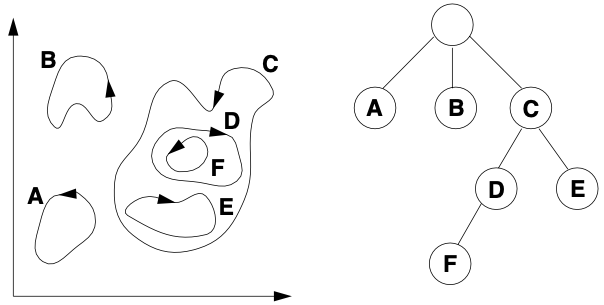
\includegraphics[width=0.45\textwidth]{hie.png}
    \caption{A set of trimming curves and the resulting hierarchy}
\end{figure}

Since the curves are not allowed to cross, there are only three possible relationships between two curves $\mathbf{c}_1$ and $\mathbf{c}_2$. $\mathbf{c}_1$ can contain $\mathbf{c}_2$, be contained in $\mathbf{c}_2$, or share no regions in common with $\mathbf{c}_2$. Each node in our hierarchy is a list of trims, and each trim can refer to yet another list of trims which fall inside of it. Building the hierarchy proceeds as:
\begin{figure}[htbp]
    \centering
    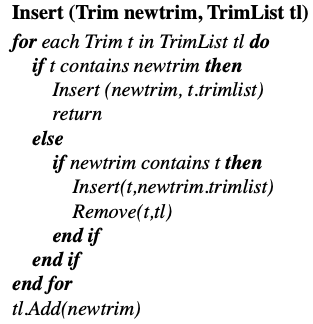
\includegraphics[width=0.3\textwidth, height=0.3\textwidth]{algo1.png}
\end{figure}

where \textit{trimlist} refers to all the child nodes of the present node.

\subsection{Root Checking}
\hspace*{8pt}
We ray trace trimmed NURBS by first performing ray intersection with the untrimmed surface. If an intersection point $\left(u_*, v_*\right)$ is found, we then look to the trim hierarchy to determine whether it is to be culled or returned as a hit. The algorithm can be described as:
\begin{figure}[htbp]
    \centering
    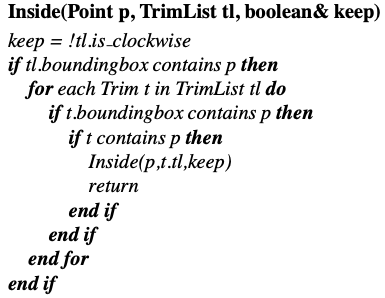
\includegraphics[width=0.3\textwidth, height=0.25\textwidth]{algo2.png}
\end{figure}

\subsection{Containment Checking}
\hspace*{8pt}
In the algorithm shown above, a problem is yet to be solved, that how to determine whether a point $(u_*,v_*)$ is inside a trimming loop. It can be solved by using a corollary of the Jordan curve theorem and the Bezier clipping algorithm. The Bezier clipping algorithm determines if a ray intersects a collection of NURBS trimming curves an even or odd number of times with high robustness. The algorithm begins by splitting the patch parameter plane into quadrants which meet at the point $\mathbf{S} = (s, t)$ as shown in Fig. 5, 

\begin{figure}[htbp]
    \centering
    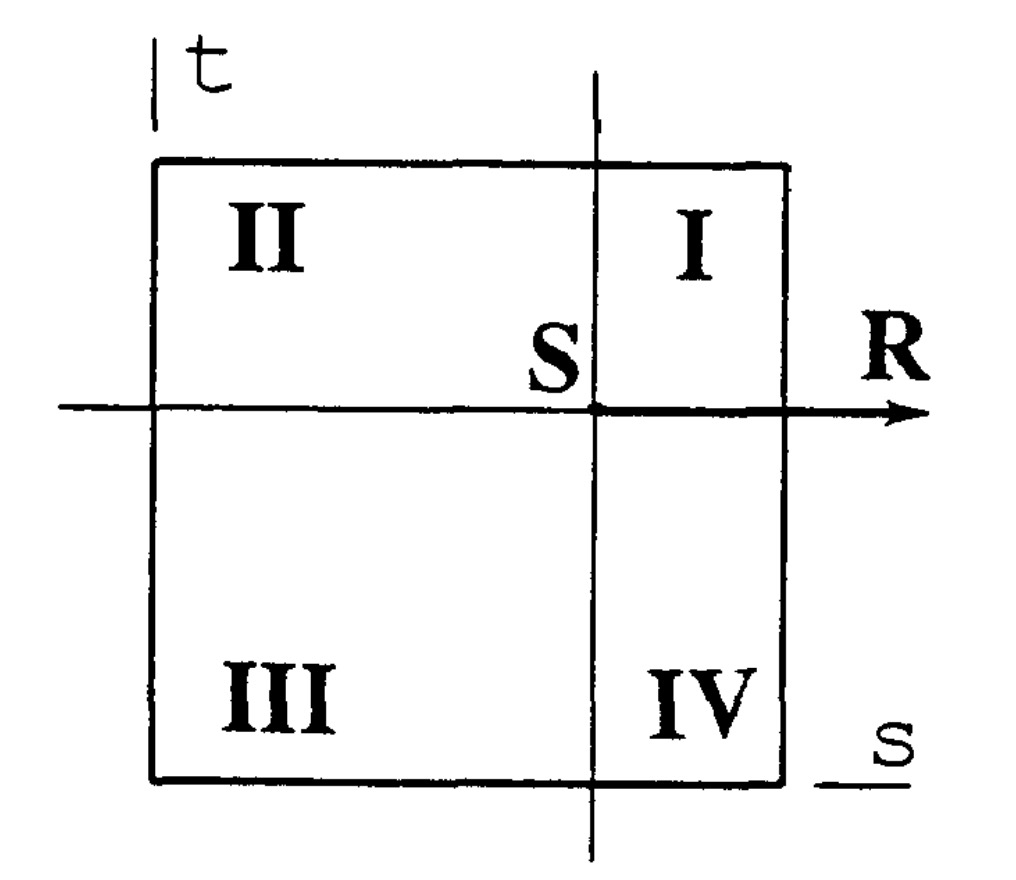
\includegraphics[width=0.3\textwidth, height=0.25\textwidth]{quadrants.png}
    \caption{Quadrants}
\end{figure}

. To determine if $\mathbf{R}$ (the ray) intersects a given NURBS trimming curve an even or odd number of times, we categorize the curve based on which quadrants its control points occupy. For now, assume that no end control point lies on a quadrant boundary.

\begin{itemize}
    \item CASE $\mathcal{A}$ : All control points lie on the same side of the line containing $\mathbf{R}$ (in quadrants I, II, III, IV, I\&II, or III\&IV) or "behind" $R$ ( in quadrants I\&III). The convex hull property of NURBS curves guarantees zero intersections with $\mathbf{R}$.
    \item CASE $\mathcal{B}$ : All control points lie in quadrants I\&IV, but not case $\mathcal{A}$. Since the curve is continuous and obeys the convex hull property, if the curve endpoints lie in the same quadrant, the curve crosses $\mathbf{R}$ an even number of times. Otherwise, the curve intersects $\mathbf{R}$ an odd number of times. Note that tangencies between the ray and trimming-curve tangencies, even those of high order, do not pose a problem. The only question is whether the curve endpoints straddle the ray.
    \item CASE $C:$ All other curves.
\end{itemize}

If a curve is case $\mathcal{A}$ or $\mathcal{B}$ no further processing is needed to determine its intersection parity with a ray. For a case $\mathcal{C}$ curve, we subdivide it using the de Boor's algorithm into three NURBS segments in such a way that the two end segments are guaranteed a priori to be case $\mathcal{A}$ or $\mathcal{B}$. Then we can easily determine whether $\mathbf{S} = (s, t)$ is in a closed NURBS trimming curve or not.

\section{Results}
For the untrimmed NURBS surface rendering, we successfully render different models. The duck only consists of three NURBS surface patches. For a single NURBS model, the scene is rendered with resolution $600\times 600$ and samples-per-pixel (spp) $256$. For the scene with 25 ducks, we set resolution be $300\times 300$, and spp be $1024$, which helps for noise reduction.
\begin{figure}[htbp]
    \centering
    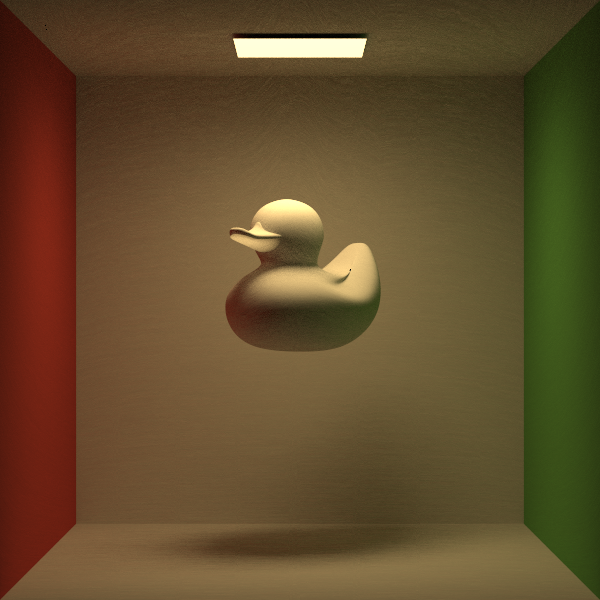
\includegraphics[width=0.45\textwidth]{../results/duck.png}
    \caption{Single duck with 3 NURBS surface patches}
\end{figure}
\begin{figure}
    \centering
    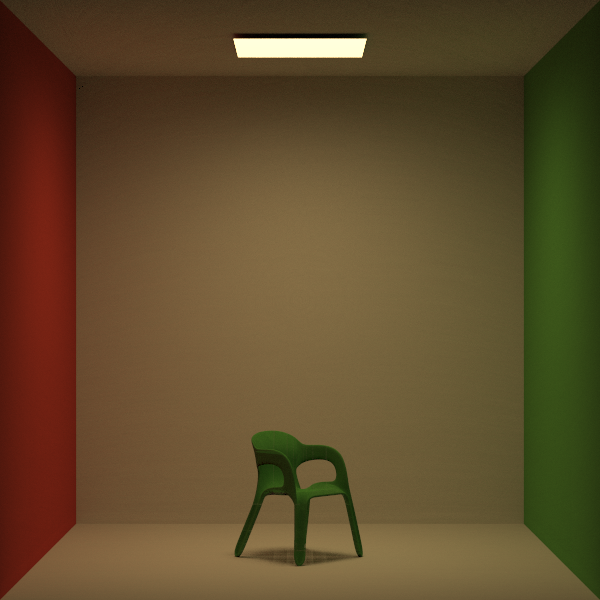
\includegraphics[width=0.45\textwidth]{../results/chair.png}
    \caption{Chair with 75 NURBS surface patches}
\end{figure}
\begin{figure}
    \centering
    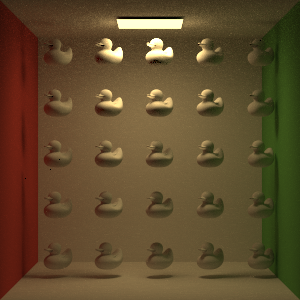
\includegraphics[width=0.45\textwidth]{../results/multi-duck.png}
    \caption{Multiple ducks with 75 NURBS surface patches in total}
\end{figure}

\section{Workload Distribution}
\hspace*{8pt}
The project workload is about evenly distributed to our two guys. The most basic part, path tracer with global illumination and BVH, is directly adopted from the code of Homework 4.

For the untrimmed NURBS part, Zeen Chi is responsible for the knot refinement algorithm and Newton's iteration implementation, and Wenchao Li is responsible for generating subdivided control points as well as Bezier patches together with their AABBs. Also, Wenchao Li tried to build a kd-tree to maintain the AABBs of each NURBS surface.

For the trimmed NURBS part, Zeen Chi is responsible for building the relative skeleton, calculating the orientation of each trimming curve, and building a hierarchy to record the relationship of containment between trimming loops. Wenchao Li is responsible for thinking about how to determine if a point $(u,v)$ is inside a trimming loop. This is extremely difficult, and we have limited time, so he will finish it afterwards if possible.

\end{document}
